\subsection[Technologien und Entscheidungen]{Technologien und Entscheidungen
 \\ \textnormal{\small{\textit {Verfasst von Victor Schwartz}}}} \label{sec:technologien}

Aus den Anforderungen heraus wurde sich im Rahmen dieser Arbeit für diverse Technologien entschieden, welche eine Umsetzung der Anforderungen des Prototypen ermöglichen.
%Eine dieser Anforderungen ist es, die Funktionen über ein Smartphone zu nutzen. Um möglichst vielen Anwendern die %Möglichkeit der Nutzung zu geben, fiel die Wahl auf Phonegap und Apache Cordova.

%TODO: Einleitung

Eine Hauptanforderung für die prototypische Umsetzung einer LBS Applikation ist 
die Lauffähigkeit auf einem Smartphone. Diese Anforderung fällt nicht weiter auf, 
ist aber entscheidend für die Auswahl der zu nutzenden Technologien.

Möchte man eine Applikation für Smartphones entwickeln, muss man sich erst Gedanken 
darüber machen, welche Smartphones bzw. mobilen Betriebssysteme unterstützt 
werden sollen.

Unterschieden wird meist nur zwischen drei Betriebssystemen, da diese die größten 
Marktanteile besitzen (Siehe Abbildung \ref{fig:Marktanteile mobiler Betriebssysteme}). 

\begin{figure}
  \centering
    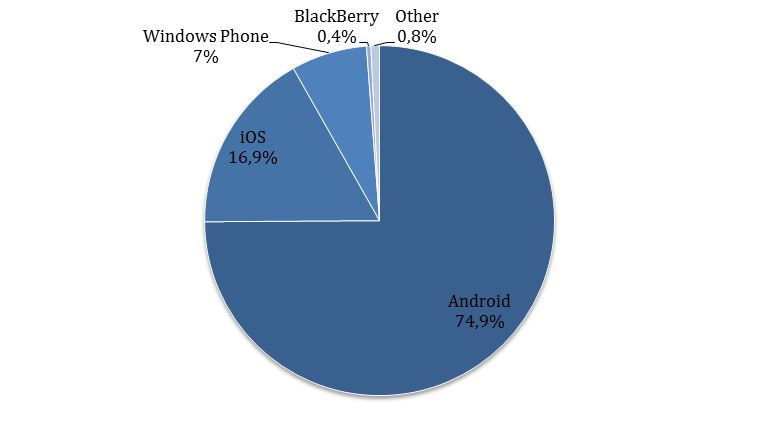
\includegraphics[width=1\textwidth]{ref/images/marktanteil.jpg} 
   \caption{Marktanteile mobiler Betriebssysteme}
  \label{fig:Marktanteile mobiler Betriebssysteme}
  \cite{Marktanteil}
\end{figure}

Es handelt sich um folgende Betriebssysteme: 
\begin{description}
  \item[$\bullet$] Android
  \item[$\bullet$] iOS
  \item[$\bullet$] Windows
\end{description}


Um den Implementieraufwand geringer zu halten, wurde entschieden die Applikation auf den zwei Betriebssystemen mit dem größten Marktanteil lauffähig zu halten. 
Android und iOS haben gemeinsam einen Anteil von über 50 Prozent. Aus dieser 
Anforderung ergaben sich drei verschiedene Möglichkeiten zur Entwicklung:
\begin{itemize}
\item Implementierung als WebApp:
 Bei dieser Art von Programm handelt es sich um eine Webseite, die für mobile 
Geräte optimiert ist.
\item Implementierung des Programm als native App: 
Bei einer nativen App handelt es sich um ein Programm, das speziell für ein mobiles Betriebssystem entwickelt wurde.
\item Implementierung als HybridApp: 
Eine HybridApp ermöglicht es mit einem Quellcode mehrere App's erstellen zu lassen. 
Zur Verwendung kommen dabei Web-Technologien.
\end{itemize}

Diese drei Möglichkeiten sollen im folgenden Abschnitt anhand von definierten 
Kriterien bewertet werden.


Folgende Kriterien wurden für die Auswahl einer Methode betrachtet:
\begin{enumerate}
\item \underline{Zugriff auf Hardware des Mobiltelefons}
\\Zur Implementierung einer LBS Applikation wird der eigene Standort benötigt. Um 
diesen zu bestimmen gibt es mehrere Verfahren. 
Die dafür benötigten Informationen sind über die Hardware des 
Smartphones erreichbar. Beispielsweise kann der Standort über den eingebauten GPS-
Empfänger bestimmt werden. Für die Implementierung der App ist es von Nöten, dass 
diese Informationen ausgelesen werden können.

\item \underline{Voraussetzungen und Vorkenntnisse}
\\Da diese Studienarbeit innerhalb von wenigen Monaten entstanden ist und andere Projekte 
parallel bearbeitet werden mussten, ist ein Kriterium über welche Vorkenntnisse die 
Entwickler verfügen. Dieses Kriterium betrachtet die eingesetzten 
Programmiersprachen und technischen Geräte, die benötigt werden um eine LBS-App 
entwickeln zu können.


\item \underline{Aufwand}
\\Dieses Kriterium ergänzt das vorhergehende. Lässt sich aber auch klar abgrenzen. Da die Zeit für diese Studienarbeit begrenzt ist, darf die Implementierung nicht zu 
viel Zeit in Anspruch nehmen, da sonst die Anforderungen nicht umgesetzt werden 
können. Betrachtet wird hierbei der Aufwand um die Anforderungen zu 
Implementieren und die App betriebssystemunabhängig zu entwickeln.
\end{enumerate}

\textbf{\underline{WebApp}}\\
Bei einer WebApp (Webapplikation) handelt es sich um eine Anwendung, die im 
Browser ausgeführt wird. Eine für Smartphones optimierte WebApp fokussiert sich 
darauf die Darstellung für kleine Bildschirme zu optimieren. Auch wird darauf 
geachtet, dass diese mit einem Touchscreen bedient werden kann. Ziel ist es, dass 
der Benutzer kaum einen Unterschied zu einer nativen App erkennt. Berechnungen 
werden bei dieser Variante meist serverseitig durchgeführt. 

\begin{enumerate}
\item Kriterium: Zugriff auf Hardware-Komponenten

Ein Nachteil der Webapplikation ist, dass nicht alle Hardware Komponenten des Smartphones angesteuert werden können.
Für die prototypische Umsetzung ist dies aber von Nöten, neben dem Standort, welche bereit gestellt werden kann, wird die Bluetooth-Komponente benötigt um iBeacons nutzen zu können.

\item Kriterium: Voraussetzungen und Vorkenntnisse

Da es sich um eine Webseite handelt, kommen die bekannten Technologien zur 
Entwicklung zum Einsatz. Hierzu zählen:HTML Hypertext Markup Language, Casscading 
Stylesheets und JavaScript.

Durch die an der dualen Hochschule erworbenen Kenntnisse in den Vorlesungen Web 
Engineering und Software Engineering, sind erweiterte Vorkenntnisse über diese 
Technologien bei allen Entwicklern dieser Arbeit vorhanden und stellen kein Problem 
dar. Zur Entwicklung reicht ein Editor sowie ein Internetbrowser. 

\item Kriterium: Aufwand

Betrachtet man die aufgezählten Technologien und Werkzeuge, so ist der Aufwand für 
die Entwicklung einer LBS-WebApp gering. Auch die Plattformunabhängigkeit stellt 
für eine WebApp keine Schwierigkeiten dar, da die genannten Web Technologien 
standardisiert sind. Allerdings fehlen definierte Schnittstellen für die Hardware-Ansteuerung, dies erhöht den Aufwand enorm.
\end{enumerate}

%http://www.sepia.de/webanwendungen-vs-mobile-apps.html

%http://www.smart-digits.com/2012/02/native-app-oder-web-app-teil-1-definitionen-
%und-entscheidungskriterien/



\textbf{\underline{Native App}}\\
Bei nativen Apps handelt es sich um Programme, welche für ein spezifisches, mobiles 
Betriebssystem optimiert und lauffähig sind. Eine Ausführung auf einem Computer oder anderem 
Betriebssystem ist, wenn überhaupt, nur schwer umsetzbar.
Installiert werden kann dies über einen betriebssystemabhängigen Marktplatz. Wie 
bereits in der Anforderungen erwähnt, soll die Applikation auf iOS und Android 
Geräten verfügbar sein, weshalb die zu untersuchenden Kriterien für beide 
Betriebssysteme betrachtet werden.

\begin{enumerate}
\item Kriterium: Zugriff auf Hardware-Komponenten

Sowohl Android wie auch iOS unterstützen einen Zugriff auf die Hardware. 
Dieser erfolgt über APIs (Applikation Programming Interface) und bietet alle mit 
dem Gerät zur Verfügung stehenden Funktionalitäten an.

\item Kriterium: Voraussetzungen und Vorkenntnisse

Android Entwicklung:
Die Programmiersprache für native Android Apps ist Java. Durch die Vorlesung Java 
Programmierung sind erweiterte Kenntnisse vorhanden. Zur komfortablen Entwicklung 
werden eine Entwicklungsumgebung (z.B. Eclipse), das aktuelle Java SDK (Software 
Development Kit) und Android SDK benötigt. Alle diese Komponenten sind kostenfrei 
verfügbar.

iOS Entwicklung:
Die Programmiersprache für native iOS Apps ist Objective-C. Zwar sind Kenntnisse 
über die Sprache C von zwei Entwicklern vorhanden, allerdings ist die Sprach C nur 
bedingt mit Objective-C vergleichbar. Es sind auf Grund dessen nur minimale 
Kenntnisse vorhanden.

Zur Implementierung einer iOS App wird neben einem Apple Computer diverse Software 
benötigt. Hierzu zählt die Entwicklungsumgebung Xcode. Möchte man die App auf einem 
Gerät testen, so wird ein Apple Developer Account, sowie das IOS Developer Programm benötigt, 
dieses ist kostenpflichtig.



\item Kriterium: Aufwand

Möchte man eine App für beide Betriebssysteme erstellen, so muss jede App einzeln 
geschrieben werden. Es kann kein Code wiederverwendet werden, da sich die 
Programmiersprachen unterscheiden. Ebenfalls sind andere APIs vorhanden, was die 
Entwicklung erschwert. Der Aufwand ist hierbei so hoch wie für zwei Apps. 
\end{enumerate}

\textbf{\underline{Hybrid App}}\\
Laut Duden ist die Definition für den Begriff Hybrid "gemischt". Dies ist auch bei solchen Apps der Fall. Mit bekannten Web-Technologien wird der Code für die Apps geschrieben. Ein Framework übernimmt im Anschluss daran, die Generierung der nativen Apps.  
\begin{enumerate}
\item Kriterium: Zugriff auf Hardware-Komponenten

Es gibt verschiedene Frameworks um eine Hybride App zu entwickeln, deshalb kann man nicht pauschal sagen welche Zugriffe auf Hardware-Komponenten möglich sind. Allerdings bieten bekannte Frameworks wie Angular UI, Intel XDK oder Adobe Phonegab eine direkte Ansteuerung an Komponenten an. Hierzu zählen beispielsweise Kamera, Kompass, Beschleunigungssenesor. Realisiert wird der Zugriff über APIs. Neben dem mitgelieferten APIs der Frameworks gibt es Plug-Ins welche von anderen Entwicklern zur Verfügung gestellt werden. Damit haben Hybrid Apps Zugriff auf eine Vielzahl von Hardware-Komponenten.

\item Kriterium: Voraussetzungen und Vorkenntnisse

Entwickelt werden Hybrid Apps mit Web Technologien. Diese sind bereits bei Kriterium 2 von WebApps behandelt worden, ebenfalls die Vorkenntnisse.

Zu den Voraussetzungen zählt die Installation von Software. Ein Framework wird benötigt. Diese unterscheiden sich in den bereitgestellten Funktionalitäten. Zur Entwicklung mit Web-Technologien wird mindestens ein Editor benötigt. Damit das Framework native Apps generieren kann, wird für die diversen Betriebssysteme SDKs benötigt. Außerdem ist es hilfreich ein Gerät pro Betriebssystem zu besitzen, um die App zu testen. Ein andere Möglichkeit ist der Einsatz eines Emulators, der ein Smartphone auf dem PC simuliert.

Alle diese Werkzeuge können kostenlos heruntergeladen werden.
%TODO: klappt das mit Apple auch


\item Kriterium: Aufwand

Möchte man eine App für verschiedene Betriebssysteme entwickeln und den Aufwand gering halten, eignen sich dafür Hybrid Apps. Neben der eigentlichen Entwicklung ist es mit Aufwand verbunden alle Werkzeuge zu installieren und zu konfigurieren. Hat man diese Hürde geschafft, ist der Aufwand gering zu bewerten. Ist die Implementierung abgeschlossen, muss dem Framework mitgeteilt werden, welche Apps gebildet werden sollen und der Rest funktioniert automatisch. Der Gesamtaufwand für die Entwicklung einer Hybrid App ist niedrig bis mittel einzustufen.
\end{enumerate}

\textbf{\underline{Zusammenfassung und Fazit}}\\

%WebApp
%Vorkenntnisse vorhanden
%Aufwand ist gering
%Hardware nicht komplett unterstützt

%Native App
%sehr wenig Vorkenntnisse, was viel Zeit in Anspruch nehmen würde
%Aufwand ist sehr hoch, weil man sich in zwei Sprachen einarbeiten muss
 %Dafür volle Hardware zur Verfügung

%Hybrid app
%Vorkenntnisse vorhanden
%Hardware meist unterstützt ansonsten Plug-Ins
 %Aufwand ist mittel bis gering

%Fazit IN dieser Arbeit wird eine Hybrid umgestetzt, da unerfahren was Frameworks angeht und meiste entwicklung mit %Cordova und Plug ins  Wahl fiel auf Apache Cordova mit Ionic

Fasst man die gewonnen Erkenntnisse über die Technologien zusammen ergibt sich folgende Tabelle:

\begin{table}[htbp]
\begin{center}
\begin{tabular}{|p{3.5cm}|p{3.5cm} p{3.5cm} p{3.5cm}|} 
	\hline
		\rowcolor{black} & \textcolor{white} { \textbf{Web App} } & \textcolor{white}{\textbf{Native App}} & \textcolor{white}{\textbf{Hybrid App}}\\ 
		\rowcolor[gray]{.75}  Zugriff auf Hardware & Nur auf wenige Hardware Komponenten kann zugegriffen werden & Voller Zugriff auf gesamte Hardware möglich & Zugriff auf Hardware durch Framework und externe Plug-Ins möglich\\ 
		\rowcolor[gray]{.9} Vorraussetzungen und Vorkentnisse & Durch die Vorlesung "Web Engineering" sind ausreichend Kentnisse vorhanden & Kentnisse für Android Programmierung durch Java vorhanden. Kentnisse über iOS Programmierung nicht vorhanden & Hybrid App wird mit Web Technologien programmiert, welche vorhanden sind. \\ 
		\rowcolor[gray]{.75} Aufwand & Gering, da eine Webseite auf alles Betriebssystem lauffähig ist & Hoher Aufwand, da zwei unabhängige native Apps entwickelt werden müssen & Gering, es wird eine App geschrieben welche auf mehreren Betriebssysteme lauffähig ist, wie beispielsweise Android und iOS \\ \hline
	\end{tabular}
\end{center}
\caption{Zusammenfassung } \label{Zusammenfassung }
\end{table}


Betrachtet man Tabelle \ref{Zusammenfassung } wird deutlich, dass eine Möglichkeit am besten zu dieser Studienarbeit passt, die Umsetzung des Prototypen als Hybrid App.
Eine Hybrid App vereint die Vorteile der WebApp mit den Vorteilen einer nativen App. Durch den schlechten Hardware Zugriff der Web App ist die Möglichkeit ungeeignet. Bei einer nativen App ist der Aufwand zu groß, da für jedes Betriebssystem eine eigene App implementiert werden muss. Durch Plug-Ins bietet eine HybridApp viele Möglichkeiten, die Hardware von Smartphones anzusteuern. Über ein Framework kann in wenigen Minuten der geschriebene Quellcode für mehrere Betriebssysteme genutzt werden um ein App zu generieren.
Aus diesen Gründen ist der Prototyp als Hybride App entwickelt worden. Verwendet wurde ein Framework von Adobe, dieses wird im nächsten Abschnitt erläutert. Drauf aufbauend findet eine kurze Vorstellung der verwendeten Web Technologien statt. 



\subsubsection[Phonegap und Apache Cordova]{Phonegap und Apache Cordova
 \\ \textnormal{\small{\textit {Verfasst von Melanie Hammerschmidt}}}}

PhoneGap entstand als Framework zur Entwicklung von Apps auf Basis von Web-Technologien wie HTML, CSS und JavaScript. 2011 wurde die Firma Nitobi Software, die PhoneGap einst entwickelte, von Adobe Systems aufgekauft, die das Produkt weiter unter dem Namen Apache Cordova fokussierten. \\
Im Rahmen der hier vorgestellten Arbeit wurde Cordova genutzt, um eine hybride App zu entwickeln. Da der Vorteil des Frameworks vor allem aus seiner Wiederverwendbarkeit besteht. Der geschriebene HTML-, CSS- und JavaScript-Code kann nämlich über Cordova entsprechend der verschiedenen Mobilplattformen unterschiedlich transformiert werden, um die entsprechende Applikation im richtigen Format zu erstellen. Unterstützt werden dabei die verbreitetsten Betriebssysteme Andorid und iOS, aber auch weitere wie Windows Phones, Blackberrys oder sogar FirefoxOS. Damit ist die fertige App später für alle zuvor vorgestellten Betriebssysteme verfügbar.


\subsubsection[Ionic]{Ionic
 \\ \textnormal{\small{\textit {Verfasst von Melanie Hammerschmidt}}}}

Ein weiteres genutztes Framework ist Ionic. Es handelt sich dabei um ein HTML5-Framework, das sich um das Benutzerinterface einer Web-Applikation kümmert. Der Fokus des Frameworks liegt dabei speziell auf mobilen Endgeräten.
Ionic bietet, in Zusammenarbeit mit Angular JS, einige UI-Komponenten, die eine Oberfläche leicht in modernem Licht erscheinen lassen.

\subsubsection[HTML 5]{HTML5
 \\ \textnormal{\small{\textit {Verfasst von Victor Schwartz}}}}

Durch die Entscheidung für Cordova und Ionic ist die Verwendung von HTML5 vorgegeben. Um eine Hybride App über Cordova erstellen lassen zu können, müssen die Texte in HTML-Seiten beschrieben werden, damit sie dann bei der Erstellung interpretiert werden können. In diesem Abschnitt wird die Technologie HTML5 im Allgemeinen erläutert.

HTML steht für Hypertext Markup Language (Übersetzt: Hypertext Auszeichnungssprache). Es handelt sich um eine textbasierte Auszeichnungssprache zur Strukturierung von Elementen auf einer Webseite. 
Über Tags werden Elemente differenziert und identifiziert. Für diverse Anwendungsfälle gibt es HTML-Tags wie beispielsweise: Überschriften, Absätze, Tabellen, Grafikelemente.
Diese Tags werden mit kleiner und größer Zeichen.

HTML liegt aktuell in der 5. Version vor, weshalb der Name HTML5 gewählt wurde. Im Laufe der Zeit (1992- bis heute) wurden immer mehr Funktionen hinzugefügt. In den Anfängen von HTML war es nur möglich Text darzustellen. Mittlerweile gehören Bilder und Farben zum Standard, mit HTML5 können mittlerweile auch komplexe Animationen erstellt werden. Durch die Standardisierung von HTML durch das W3C können nahezu alle Browser in HTML5 entwickelte Webseiten anzeigen. Diese Funktionalitäten werden für den Prototypen verwendet.



\subsubsection[CSS]{CSS
 \\ \textnormal{\small{\textit {Verfasst von Victor Schwartz}}}}

CSS steht für Cascading Style Sheets (gestufte Gestaltungsbögen). Es handelt sich um eine Gestaltungssprache welche unter anderen in Verbindung mit HTML genutzt wird. CSS werden genutzt um das Design für Webseiten zu gestalten. Zu einem Design können mit CSS Farben, Formen, Schriftarten und vieles mehr gehören. Durch die Trennung von Text mit HTML und Design durch CSS ist es möglich mehrere Webseiten mit ähnlichem oder gleichen Design zu gestalten. Realisiert wird dies mit einer CSS-Datei. In einer CSS Datei sind meist mehrere Klassen vorhanden. Jede Klasse besitzt verschiedene Eigenschaften wie Farbe, Schriftart oder Schriftgröße. Möchte man diese Klassen in einem HTML Dokument verwenden, so verknüpft man die CSS-Datei mit einem speziellen Tag mit der HTML Seite und kann dann beispielsweise Textabschnitten oder Überschriften die definierten Klassen zuweisen.



%http://www.w3.org/standards/webdesign/htmlcss

\subsubsection[Angular-JS]{Angular-JS
 \\ \textnormal{\small{\textit {Verfasst von Melanie Hammerschmidt}}}}
Angular JS ist ein Framwork, das voll auf JavaScript aufbaut und komplett klientenseitig ausgeführt wird.
\\
Es ist das Framewort, welches die "'Zwei-Wege-Datenbindung"'\cite{angular} unterstützt, die in unserem Prototypen so häufig verwendet wird. Es können dabei Daten sowohl von der dargestellten Seite übergeben sowie aufgenommen und dargestellt werden. Dieser gezielte Datenaustausch macht die Applikation enorm flexibel im Aufbau und in der Nutzung und zusätzlich die Architektur deutlich einfacher und strukturierter.
\\
Außerdem werden durch Angular JS die Trennung von Darstellungssschicht (View) und Datenschichten (Controller und Model) unterstützt. Diese Trennung ist im Verlauf der Entwicklung von großer Bedeutung (vgl. Architektur). Angular JS bietet also kurz gesagt viele weitere Alternativen zu den herkömmlichen HTML-Tags. Nähere Implementierungsdetails zu Views, Controllern und Models folgen im Kapitel Implementierung.

\subsubsection[Kartenmaterial]{Kartenmaterial \label{sec:kartenmaterial}
 \\ \textnormal{\small{\textit {Verfasst von Patrick Senneka}}}}
 
Kartenmaterial im Browser bzw. einer Hybrid-App ist ein essentieller Bestandteil von Location based Services. Durch eine Positionsbestimmung alleine erhält man nur Daten die für den Nutzer nicht anschaulich sind. Diese liegen normalerweise als geografische Koordinaten vor, die in geografischer Breite und geografischer Länge angegeben werden. Eine Beispielposition soll die Bedeutung von Kartenmaterial für den Nutzer von Location based Services verdeutlichen.


Als Beispiel hierfür wurde die Position der DHBW Mannheim in der Coblitzallee gewählt. Hierbei werden die geografischen Koordinaten, eine Adresse und ein Kartenausschnitt in einer Tabelle gegenübergestellt. Siehe hierzu Tabelle \ref{BedeutungVonKartenmaterial}.

\begin{table}[htbp]
\begin{center}
\begin{tabular}{|p{4.75cm}p{4.75cm}p{4.75cm}|} 
	\hline
		\rowcolor{black} \textcolor{white} { \textbf{Geographische Koordinaten} } & \textcolor{white}{\textbf{Adresse}} & \textcolor{white}{\textbf{Kartenausschnitt}}\\ 
		\rowcolor[gray]{.75}  49$^\circ$28'27.6\grqq N 8$^\circ$32'03.9\grqq E & Duale Hochschule Baden-Württemberg Mannheim \newline 
Coblitzallee 1-9 \newline 
68163 Mannheim \newline (Neuostheim) & Kartenausschnitt\newline 

\includegraphics[width=0.3\textwidth]{ref/images/KartenmaterialKlein.png} \\ 
\hline
	\end{tabular}
\end{center}
\caption{Bedeutung von Kartenmaterial} \label{BedeutungVonKartenmaterial}
\end{table}

In der Tabelle sind verschiedenen Ortsdaten zur Verfügung gestellt, die jeweils Vor- und Nachteile aufweisen.

Die geographischen Koordinaten geben die Position am genausten an, sind aber für fast keine Nutzer einer App anschaulich und bieten deshalb keinen großen Nutzen. 

Die Adresse ist im Alltag am geläufigsten und somit für Nutzer am verständlichsten. Allerdings ist die Angabe nicht so genau wie die geographischen Koordinaten, denn die Angabe Hausnummer 1-9 gibt einen relativ großen Bereich an.

Die Vorteile eines Kartenausschnitts sind, dass die Detaillierung vom Nutzer angepasst werden kann. Des Weiteren werden viele grafische Informationen angezeigt, wie zum Beispiel den eigene Standort, an denen sich ein Nutzer orientieren kann. Der Nachteil dieser Variante ist, dass die Kartenausschnitte eine Abhängigkeit von externen Quellen und einem höheren Programmieraufwand gegenüber geographischen Koordinaten mit sich bringen.


Auf Smartphones gehört Kartenmaterial und dessen Integration in Apps mittlerweile zum Standard, an welchen sich Nutzer gewöhnt haben. Und über die Hälfte der Deutschen, 44 Millionen nutzen schon ein Smartphone. Die Tendenz ist dabei steigend. Dies ist das Ergebnis einer Bitkom Studie. \cite{bitkom} Aus diesem Grund sollte auch Kartenmaterial in die Location based Services App integriert werden, welche die Autoren bei dieser Studienarbeit prototypisch entwickeln. 

Mögliche Quellen für das Kartenmaterial sind \glqq Google Maps\grqq, \glqq Bing Maps\grqq  und \glqq Open Street Maps\grqq.

Da Kartenmaterial eine zentrale Quelle der App darstellen wird, ist die Auswahl eines Anbieters von großer Bedeutung. Aus diesem Grund wird hier eine genaue Analyse durchgeführt, welches Kartenmaterial sich am besten für diese App eignet.

\textbf{Anforderungen an das Kartenmaterial}


Die Anforderungen an interaktives Kartenmaterial, bezüglich der in dieser Studienarbeit entwickelten App, lassen sich in zwei Gruppen einteilen, die funktionalen und nichtfunktionalen Anforderungen.

Die \underline{nichtfunktionalen Anforderungen} sind:
\begin{enumerate}
\item Kostenlose Abfragen
\item Ohne Account nutzbar
\item Gute Dokumentation mit Codebeispielen
\end{enumerate}

Die \underline{funktionalen Anforderungen} an das interaktive Kartenmaterial sind:
\begin{enumerate}
\item JavaScript API
\item Unterstütze Browser
\item Eigenen Standort anzeigen
\item Markierungen auf der Karte setzen
\item Markierungen bündeln (optional)
\end{enumerate}

Bevor \glqq Google Maps\grqq, \glqq Bing Maps\grqq  und \glqq Open Street Map\grqq  bezüglich der Anforderungen untersucht werden, müssen diese genauer spezifiziert werden.

Zuerst widmen wir uns den nichtfunktionalen Anforderungen.
\begin{enumerate}
\item Kostenlose Abfragen \\
Da es sich bei der Implementierung um einen Prototypen für diese Studienarbeit handelt und dieser nicht kommerziell verwendet werden soll, sollen auch die Abfragen (map-loads) kostenlos sein. Zudem sollten genug kostenlose Abfragen zur Verfügung stehen. Bei drei Entwicklern und Tests über die Dauer der Studienarbeit (8-9 Monate) darf das Kontingent der kostenlosen Abfragen nicht aufgebraucht sein.

\item Ohne Account nutzbar\\
Die Nutzung ohne Account vereinfacht den Einstieg für das Kartenmaterial und sollte deshalb gewährleistet sein. 
%Zudem würden dann alle Teammitglieder dieser Studienarbeit mit dem selben Account eines Teammitglieds arbeiten. 

\item Gute Dokumentation mit Codebeispielen\\
Eine gute Dokumentation der API des Kartenmaterials mit vielen Codebeispielen erleichtert den Einstieg deutlich. Da die Teammitglieder dieser Studienarbeit zu Beginn noch keine Erfahrung mit Kartenmaterial hatten, ist dies eine besonders wichtige Anforderung. 


\end{enumerate}



Als nächstes werden die funktionalen Anforderungen genauer erläutert.

\begin{enumerate}
\item JavaScript API\\
Eine JavaScript API ist essentiell wichtig, da der Prototyp mit HTML, CSS und Java Script entwickelt wird. 

\item Unterstütze Browser\\
Als unterstützte Browser sollten die Browser von den drei großen Smartphone-Betriebssystemen Android, IOS und Windows Phone unterstützt werden, um sich die Möglichkeit offen zu halten die prototypische App auch auf anderen Plattformen zu nutzen.

\item Eigenen Standort anzeigen\\
Der eigene Standort muss grafisch auf einer interaktiven Karte angezeigt werden. Das Zentrieren des Kartenmaterials auf den eigenen Standort soll zudem möglich sein.

\item Markierungen auf der Karte setzen\\
Eigenen Markierungen müssen auf der Karte gesetzt werden könne. Dies muss grafisch erfolgen, denn es ist für den Prototypen besonders wichtig zu veranschaulichen, in welchem Bereich sich Ziele befinden. 

\item Markierungen bündeln (optional)\\
Markierungen auf der Karte sollten gebündelt werden, wenn der Zoom-Faktor zu klein wird. Dies soll der Übersichtlichkeit bei vielen Markierungen auf der Karte dienen. Hierbei soll der Radius, in dem Markierungen gebündelt werden, eingestellt werden können.

Diese Anforderung ist als optional gekennzeichnet, da eine Bündelung erst bei vielen Zielen zu Übersichtlichkeit nötig ist und zunächst einmal mit wenig Zielen entwickelt wird.

\end{enumerate}



\textbf{\underline{Google Maps}}\\

Seit 2005 gehört zu dem Produktportfolio von dem Suchmaschinenriesen Google ein Internet-Kartendienst namens Google Maps. 
Er gehört zu den verbreitetsten und erfolgreichsten Internet-Kartendiensten der Welt. \cite[Lexikon Google Maps]{itwissen}\cite[S.88]{gruber2015}

Zunächst wird Google Maps anhand der nichtfunktionalen Anforderungen bewertet, danach werden die funktionalen Anforderungen betrachtet.

\textbf{Nichtfunktionale Anforderungen}
\begin{enumerate}
\item Kostenlose Abfragen \\
Die Google Maps API steht generell als kostenloser Dienst zur Verfügung. Dieser darf in Webseiten, sowie mobile Apps eingebaut werden. Als Voraussetzung für die kostenlose Nutzung gilt allerdings, dass die eigene Webseite oder mobile App für alle Endnutzer kostenlos ist und öffentlich zugänglich sein muss.\\
Unter der kostenlosen Lizenz dürfen bis zu 25.000 Kartenladevorgänge pro Tag erfolgen. Ein Kartenladevorgang ist als initiales Laden der Karte definiert. Das bedeutet, dass Nutzerinteraktion mit der Karten nicht als erneuter Ladevorgang gewertet wird. 
In den Nutzungsbedingungen von Google wird darauf verwiesen, dass eine Sperre von mehr als 25.000 Abfragen pro Tag erst dann durchgeführt wird, wenn die Begrenzung mehr als 90 Tage in Folge überschritten werden sollte.
Diese Auslegung erscheint sehr nutzerfreundlich. Für diese Studienarbeit sollten die 25.000 Abfragen pro Tag in jedem Fall ausreichen. \cite[Nutzungsbedingungen]{googlemaps}\cite[Lizenzierung]{googlemaps}


\item Ohne Account nutzbar\\
Seit dem die Google Maps JavaScript API in der Version 3 vorliegt ist die Nutzung ohne einen Schlüssel möglich. Das bedeutet, dass keine Registrierung bzw. Anmeldung zum Nutzen nötig ist. Diese Praxis erleichtert es den Einstieg in Google Maps, da man sofort starten kann. \cite{googlemapsblog}


\item Gute Dokumentation mit Codebeispielen\\
Google Maps bietet ein Entwicklerhandbuch für die JavaScript API v3, dass sowohl ausführlich ist, als auch viele Beispiele bietet. Zudem ist das Benutzerhandbuch in deutsch abrufbar, was das Erarbeiten und Nachlesen vereinfacht. 
Zum ausführlichen Entwicklerhandbuch gibt es nochmals fast 150 Beispiele, zu denen der jeweils passende Output (Karte) angezeigt wird.\cite[Documentation]{googlemaps} \\
Neben der Dokumentation von Google selbst gibt es auch andere Tutorials im Netz. Eines davon ist von der Webseite www.w3schools.com, dass versucht von Grund auf eine Einführung in Google Maps zu geben. 



\end{enumerate}


\textbf{funktionale Anforderungen}
\begin{enumerate}
\item JavaScript API\\
Mit der Google Maps JavaScript API Version 3 bietet Google eine JavaScript API die sich sehr leicht in Webseiten integrieren lässt. 

Bei HTML muss lediglich ein Skript Tag eingefügt werden, in dem als Quelle (src) die Google Maps API zu finden ist. Vergleiche Listing Zeile 1. Danach können mit JavaScript Karten von Google Maps erstellt werden. Vergleiche Listing Zeile 2 - 12.
\begin{lstlisting}
<script src="https://maps.googleapis.com/maps/api/js?v=3.exp"></script>
    <script>
		var map;
		function initialize() {
		  var mapOptions = {
		    zoom: 8,
		    center: new google.maps.LatLng(-34.397, 150.644)
		  };
		  map = new google.maps.Map(document.getElementById('map-canvas'),
	      mapOptions);
		}
		google.maps.event.addDomListener(window, 'load', initialize);
    </script>
\end{lstlisting} \cite[Codebeispiel Simple Map]{googlemaps}


\item Unterstütze Browser\\
Von der Google Maps JavaScript API 3 werden fast alle gängigen Browser unterstützt. Diese sind:

\glqq 
    IE 7.0 und höher (Windows)
    
    Firefox 3.0 und höher (Windows, Mac OS X und Linux)
    
    Safari 4 und höher (Mac OS X und iOS)
    
    Chrome (Windows, Mac OS X und Linux)
    
    Android
    
    BlackBerry 6
    
    Dolfin 2.0 und höher (Samsung Bada)
\grqq \cite{googlemaps}

Die offizielle Unterstützung des Windows Phone Internetexplorers fehlt hierbei.

\item Eigenen Standort anzeigen\\
Den eigenen Standort kann man, sofern dieser bestimmt werden konnte (Listing Zeile 1 - 5), mit der Google Maps API auf der Karte anzeigen. Dies kann man zum Beispiel mit einer Informationsbox, die man mit \glqq new google.maps.Infowindow \grqq auf dem eigenen Standort erstellt, erfolgen. (Listing Zeile 7 - 11) Zur besseren Veranschaulichung wird die Karten dann noch auf die eigene Position zentriert (Listing Zeile 13)

\begin{lstlisting}
  // Try HTML5 geolocation
  if(navigator.geolocation) {
    navigator.geolocation.getCurrentPosition(function(position) {
      var pos = new google.maps.LatLng(position.coords.latitude,
                                       position.coords.longitude);

      var infowindow = new google.maps.InfoWindow({
        map: map,
        position: pos,
        content: 'Location found using HTML5.'
      });

      map.setCenter(pos);
    }
\end{lstlisting} \cite[Codebeispiel Geolocation]{googlemaps}

\item Markierungen auf der Karte setzen\\
Markierungen könne mit der API sehr leicht gesetzt werden. Neben der Position der Markierung muss noch eine Referenz auf die Google Maps Karte, sowie ein Name bei der Erstellung angegeben werden. Vergleiche Listing:

\begin{lstlisting}
  var marker = new google.maps.Marker({
      position: new google.maps.LatLng(-25.363882,131.044922),
      map: map,
      title: 'Hello World!'
  });

\end{lstlisting} \cite[Codebeispiel Simple Markers]{googlemaps}

Den Markierungen auf der Karte können auch Bilder mit dem Attribut \glqq icon \grqq zugeordnet werden. Des Weiteren kann man mit dem Attribut \glqq draggable \grqq einstellen, ob man die Markierung verschieben kann oder nicht.

\item Markierungen bündeln (optional)\\
Markierungen können in der Standard JavaScript API in Version 3 nicht gebündelt werden. 

Mit einer zusätzlichen Bibliothek  von Google kann diese Funktionalität allerdings ergänzt werden. Die Bibliothek heißt \glqq google-maps-utility-library-v3 \grqq. 
Mit Hilfe dieser Bibliothek kann ein \glqq Markercluster \grqq erstellt werden, dass Markierungen bei einer gewissen Zoomstufe bündelt. Hierbei wird dem Markercluster ein Array der Markierungen, eine Refernz auf die Karte, sowie Markercluster-Einstellungen übergeben.
%TODO: Formulierung an Listing anpassen ? markers anstatt Markierungen

\begin{lstlisting}
var mcOptions = {gridSize: 50, maxZoom: 15};
var markers = [...]; // Create the markers you want to add and collect them into a array.
var mc = new MarkerClusterer(map, markers, mcOptions);
\end{lstlisting}
\cite{googlecluster}

\end{enumerate}





\textbf{\underline{Bing Maps}}\\
Bing Maps ist der Kartendienst des Softwarekonzerns Microsoft. Neben Kartenmaterial bietet der internet-basierte Dienst auch Satellitenbilder und Luftaufnahmen.

\textbf{Nichtfunktionale Anforderungen}
\begin{enumerate}
\item Kostenlose Abfragen \\
Bing Maps bietet für öffentlich zugängliche Webseiten, sowie für mobile Apps für Konsumenten ein kostenloses Kontingent von 125.000 Transaktionen pro Jahr. Will man dieses Kontingent von Transaktionen überschreiten, werden Kosten fällig.
\cite{microsoft}

\item Ohne Account nutzbar\\
Bing Maps ist nicht ohne einen Account nutzbar. Bevor man mit der dazugehörigen API entwickeln kann, ist es nötig zuerst eine Microsoft ID anzulegen, mit der man dann wiederum einen Entwickler Key für Bing Maps anfordern kann. Ein schneller Einstieg ist auf Grund von Registrierungen nicht möglich. Zudem gibt es unterschiedliche Lizenzmodelle, die zwischen Webseite und mobile App unterscheiden, was zur Folge hat, dass man für eine neue Plattform einen neuen Key benötigt. \cite{gruber2015} \cite{microsoft}

\item Gute Dokumentation mit Codebeispielen\\
Bing Maps bietet eine ausführliche Dokumentation für die Bing Maps AJAX Control Version 7.0. Dabei werden die Klassen beschrieben und fast jede mit einem Beispiel verdeutlicht. 
Zusätzlich gibt es über 200 Codebeispiele, die man direkt im Browser ausprobieren und editieren kann. Diese Beispiele kann man auch ohne Account (Key) nutzen.

\end{enumerate}



\textbf{funktionale Anforderungen}
\begin{enumerate}
\item JavaScript API\\
Bing Maps bietet eine JavaScript API, die \glqq Bing Maps AJAX Control Version 7.0 \grqq. Es ist möglich diese einfach in einem script-Tag in eine HTML-Seite einzubinden (Listing Zeile 1). Danach kann man eine Karte erstellen, indem man ein neues Map Objekt erzeugt. (Listing Zeile 6) 
\begin{lstlisting}
<script type="text/javascript" src="http://ecn.dev.virtualearth.net/mapcontrol/mapcontrol.ashx?v=7.0"></script>
      <script type="text/javascript">
      var map = null;
      function getMap()
      {
          map = new Microsoft.Maps.Map(document.getElementById('myMap'), {credentials: 'Your Bing Maps Key'});
      }   
      </script>
\end{lstlisting} \cite[Codebeispiel CreateMap1]{bingmaps}


\item Unterstütze Browser\\
Die JavaScript API von Bing Maps wird laut Microsoft von fast allen Browsern unterstützt. 

Die unterstützen Desktop Browser sind:

\glqq
\begin{itemize}
\item Internet Explorer 7.0 and later
\item Firefox 3.6 and later
\item Safari 5 and later
\item Google Chrome
\end{itemize}

Die unterstützen mobilen Browser sind:
\begin{itemize}
\item Internet Explorer Mobile Browser
\item Apple iPhone Browser
\item Google Android Browser
\item Research in Motion (RIM) BlackBerry Browser
\end{itemize}
\grqq \cite{microsoftbrowser}

Alle relevanten Browser für Smartphones werden unterstützt.

\item Eigenen Standort anzeigen\\
Der eigene Standort kann bei Bing Maps mit einem \glqq GeoLocationProvider \grqq ermittelt werden. Dieser erhält eine Referenz auf das Kartenobjekt, in dem der Standort angezeigt werden soll (Listing Zeile 2). Mit der Funktion \glqq getCurrentPosition \grqq kann dann der Standort des Nutzers ermittelt werden.
\begin{lstlisting}
map.entities.clear(); 
var geoLocationProvider = new Microsoft.Maps.GeoLocationProvider(map);  
geoLocationProvider.getCurrentPosition(); 
\end{lstlisting}\cite[Codebeispiel GetUserLocation1]{bingmaps}

\item Markierungen auf der Karte setzen\\
Mit Bing Maps ist es möglich Markierungen auf der Karte zu platzieren. Dieser werden hierbei PushPins genannt. Diese Pushpins werden zum Anzeigen dem Map Objekt übergeben (Listing Zeile 3). Eine nachträgliche Positionsänderung der gesetzten Pushpins ist einfach möglich, indem man diesem eine neue Position zuweist (Listing Zeile 4).

\begin{lstlisting}
map.entities.clear(); 
var pushpin= new Microsoft.Maps.Pushpin(map.getCenter(), null); 
map.entities.push(pushpin); 
pushpin.setLocation(new Microsoft.Maps.Location(47.5, -122.33)); 
\end{lstlisting}\cite[Pushpins7]{bingmaps}

\item Markierungen bündeln (optional)\\
Microsoft bietet keine Funktion mit der man Markierungen(Pushpins) zusammenfassen kann. Um diese Funktionalität dennoch mit Bing Maps nutzen zu können, kann man auf Code von Drittherstellen zurückgreifen. Dieser Code kann allerdings in einer neuen Version von Bing Maps unbrauchbar sein und eine Weiterentwicklung ist nicht sehr wahrscheinlich, da hinter den Drittherstellen meist nur eine Person steht. \cite[S. 92]{gruber2015}
\end{enumerate}








\textbf{\underline{Open Street Maps}}\\
Open Street Map ist die sogenannte \glqq offenste aller Karten \grqq \cite[S.92]{gruber2015}. Das bedeutet, dass das Kartenmaterial von der OpenStreetMap Foundation jedem frei und kostenlos zu Verfügung gestellt wird. Das Kartenmaterial selbst kann von jedem Nutzer überarbeitet werden oder es kann als Basis für neues Kartenmaterial dienen (Points of Interest). So steht es auch jedem frei Fehler zu finden und verbessertes Kartenmaterial einzureichen.

Mit Open Streetmap ist es sogar möglich seine eigenen Karten zu verwenden.

Da Open Streetmap nur Karten liefert und keine dazugehörigen API's ist man auf eine API von einer anderen Quelle angewiesen. Auf der Webseite www.openstreetmap.org wird als JavaScript API LeafletJS verwendet. 
In der weiteren Betrachtung ist Open Streetmap immer unter der Verwendung von LeafletJS zu sehen.


\textbf{Nichtfunktionale Anforderungen}
\begin{enumerate}
\item Kostenlose Abfragen \\
Open Steet Map bietet jedem privaten oder Kommerziellen Nutzer die Möglichkeit auf das Kartenmaterial zuzugreifen. Abfragen sind dabei generell kostenlos. Des Weiteren ist die Anzahl der Abfragen weder für einen Tag, noch für ein Jahr begrenzt. \cite{gruber2015}


\item Ohne Account nutzbar\\
Für die Nutzung von Open Street Map ist weder eine Registrierung, noch ein Account erforderlich. Nach der Angabe der Ressource im Script Tag (Leaflet API) einer Webseite kann mit JavaScript auf das Kartenmaterial von Open Street Map zugegriffen werden. 
\cite{leaflet}

\item Gute Dokumentation mit Codebeispielen\\
Eine gute Dokumentation ist durch die Webseite von Leaflet gegeben. Alle Funktionen werden dort übersichtlich beschrieben, sowie anhand von Beispielen erläutert. 

Ein großer Vorteil der Dokumentation von Leaflet sind die Tutorials. Diese beschränken sich auf die wesentlichen Funktionen, wie beispielsweise die Nutzung von Leaflet unter mobilen Geräten. 
\cite{leaflet}

Bei schwierigen Aufgaben ist es durch Wiki-Beiträge nahezu immer diese zu lösen. \cite{gruber2015}


\end{enumerate}

\textbf{funktionale Anforderungen}
\begin{enumerate}
\item JavaScript API\\
Die OpenStreetMap Foundation selbst bietet nur Kartenmaterial an. Eine JavaScript API von der OpenStreetMap Foundation ist nicht vorhanden. Allerdings gibt es Bibliotheken, die von anderen Projekten veröffentlicht wurden, die diese Funktionalitäten abbilden. Die bekannteste dürfte \glqq Leaflet \grqq sein. Leaflet wird nämlich auch auf der Webseite von Open Steet Map, \glqq www.openstreetmap.org \grqq , genutzt.

Die API von Fremdprojekten haben zum Nachteil, dass nicht mehr alles aus einer Hand kommt.
\cite{gruber2015}

\item Unterstütze Browser\\
Leaflet untersützt Browser nahezu alle Browser. Generell werden Browser unterstützt, die unter der HTML-Rendering-Engine WebKit laufen, was schon fast alle Browser abdeckt. Die unterstützten Browser sind im einzelnen:

\glqq 
On Desktop

    Chrome,
    
    Firefox,
    
    Safari 5+,
    
    Opera 12+,
    
    IE 7–11

On Mobile

    Safari for iOS 3–7+,
    
    Android browser 2.2+, 3.1+, 4+,
    
    Chrome for Android 4+ and iOS,
    
    Firefox for Android,
    
    Other WebKit browsers (webOS, Blackberry 7+, etc.),
    
    IE10/11 for Win8 devices
\grqq
\cite{leaflet}

Alle relevanten Browser von Smartphones werden unterstützt.

\item Eigenen Standort anzeigen\\
Der Eigene Standort lässt sich mit Leaflet mit einer einzigen Funktion bestimmen. Vergleiche hierzu Listing Zeile 17. 

Um den Standort anzuzeigen ist zunächst ein Kartenobjekt nötig. Dieses wird in Zeile 1 des Listings initialisiert. Um die eigene Position auf der Karte grafisch anzeigen zu können ist die Funktion \glqq onLocationFound  \grqq, im Listing Zeile 3 bis 8,  nötig. Diese Funktion wird aktiviert, wenn der eigene Standort gefunden wurde. Dann wird die Genauigkeit des Standorts ermittelt und grafisch über einen circle dargestellt (Zeile 4 und 7). Das Zentrum des Standorts wird durch einen Marker (Zeile 5) dargestellt.

Wenn der Standort nicht bestimmt werden konnte wird dem Nutzer mit der Funktion \glqq onLocationError \grqq eine Fehlermeldung angezeigt.

\begin{lstlisting} 
var map = L.map('map');

function onLocationFound(e) {
	var radius = e.accuracy / 2;
	L.marker(e.latlng).addTo(map)
		.bindPopup("You are within " + radius + " meters from this point").openPopup();
	L.circle(e.latlng, radius).addTo(map);
}

function onLocationError(e) {
	alert(e.message);
}

map.on('locationfound', onLocationFound);
map.on('locationerror', onLocationError);

map.locate({setView: true, maxZoom: 16});
\end{lstlisting}  \cite{leaflet}

Dieses Beispiel zeigt gut, wie die Leaflet JavaScript API aufgebaut ist. Hier sind alle Funktion separat und können einzeln genutzt werden. So kann man als Programmierer genau die Funktionalitäten nutzen, die man braucht. In diesem Beispiel ist es auch möglich die Karte stets auf den eigenen Standort zu zentrieren und diesen nicht zusätzlich grafisch anzuzeigen.

\item Markierungen auf der Karte setzen\\
Markierungen können mit der Funktion \glqq marker(latitude, longitude) \grqq erstellt werden und der Karte hinzugefügt werden. Ein Beispiel dafür ist schon im Listing der Funktionalen Anforderung 3 in Zeile 5 bis 6 enthalten.

\item Markierungen bündeln (optional)\\
Mit LeafletJS lassen sich Marker nicht bündeln. Diese Funktionalität kann durch das einbinden eines weiteren Projekts, \glqq  Leaflet.markercluster \grqq ergänzt werden. \cite[S.92]{gruber2015}

Das Markercluster kann eine Sammlung von Markern auf der Karte gebündelt anzeigen. Die Marker können mit \glqq .addLayer() \grqq zum Markercluster hinzugefügt werden. Dieses wird wiederum als Layer zur Karte hinzugefügt. (Listing Zeile 6)

\begin{lstlisting}
var markers = new L.MarkerClusterGroup();

markers.addLayer(L.marker([175.3107, -37.7784]));
// add more markers here...

map.addLayer(markers);
\end{lstlisting} \cite{leaflet}

\end{enumerate}


\textbf{\underline{Fazit Kartenmaterial}}\\
Um ein Fazit zu ziehen, welches Kartenmaterial zum Einsatz in der Location-based Services App kommt, wird hierbei zuerst auf die Vor und Nachteile der einzelnen Anbieter eingegangen.

\textbf{Google}

Vorteile:
\begin{itemize}
\item Alles kommt aus einer Hand
\item Keine Registrierung nötig
\item Gute und ausführliche Dokumentation mit vielen Beispielen
\end{itemize}

Nachteile:
\begin{itemize}
\item Lizenzkosten fallen an, wenn 25000 Abfragen pro Tag häufig überschritten werden
\item Der Internetexplorer für Windows Phone wird offiziell nicht unterstützt
\end{itemize}


\textbf{Bing}

Vorteile:
\begin{itemize}
\item Gute und ausführliche Dokumentation mit vielen Beispielen
\item Alle relevanten Browser werden unterstützt
\end{itemize}

Nachteile:
\begin{itemize}
\item Cluster nur mit externer Bibliothek nutzbar
\item Registrierung ist erforderlich 
\item Unterschiedliche Lizenzmodelle für Web und mobile Anwendungen
\item Anzahl der kostenlosen Abfragen ist sehr begrenzt
\end{itemize}


\textbf{Open Street Map}

Vorteile:
\begin{itemize}
\item Unbegrenzt viele kostenlose Abfragen
\item Individualisierbarkeit(eigenes Kartenmaterial)
\item Alle relevanten Browser werden unterstützt
\item Gute und ausführliche Dokumentation mit vielen Beispielen
\item Verständliche API Struktur
\end{itemize}

Nachteile:
\begin{itemize}
\item Man ist auf mindestens 3 Hersteller bzw. Quellen angewiesen
\end{itemize}



\underline{Bewertung der nichtfunktionale Anforderungen:}
\begin{enumerate}
\item Kostenlose Abfragen: \\
OpenStreetMap bietet unlimitiert viele kostenlose Abfragen und kann damit überzeugen.
\item Ohne Account nutzbar: \\
OpenStreetMap und Google Maps können ohne Account genutzt werden.
\item Gute Dokumentation mit Codebeispielen:\\
Alle drei Anbieter bieten ausführliche Dokumentationen mit Tutorials an.
\end{enumerate}

Bei den nichtfunktionalen Anforderungen schneidet Open Steet Maps am besten ab. 

\underline{ Bewertung der funktionalen Anforderungen:}
\begin{enumerate}
\item JavaScript API:\\
Alle Anbieter bieten eine JavaScript API und überzeugen damit. Die Kapselung der Funktionen von OpenStreetMap scheint aber für die Autoren am sinnvollsten gewählt zu sein.
\item Unterstützte Browser:\\
Google Maps unterstützt den Internet Explorer für Windows Phone Geräte offiziell nicht. Bing Maps und OpenStreetMap können mit den unterstützten Browsern überzeugen.
\item Eigenen Standort anzeigen:\\
Alle drei Anbieter überzeugen hierbei gleichermaßen.
\item Markierungen auf der Karte setzen:\\
Auch hierbei überzeugen alle drei Anbieter gleichermaßen.
\item Markierungen bündeln:\\
Google Maps liefert alles aus einer Hand sowohl bei Bing Maps, als auch bei OpenStreetMap muss auf Bibliotheken dritter zurückgegriffen werden.
\end{enumerate}

Durch die fehlende offizielle Unterstützung von Google Maps für den Windows Phone Browser ist es nicht für diese Studienarbeit geeignet, da man sich die Möglichkeit offen halten möchte, eine plattformübergreifende mobile LBS App zu entwickeln.

Im Vergleich der Vor und Nachteile und den nichtfunktionalen Anforderungen überzeugt OpenStreetMaps bei den gewählten Anforderungen deutlich mehr als Bing Maps.

Das Fazit ist, dass sich OpenStreetMaps am besten für den Einsatzzweck dieser Studienarbeit und der damit verbundenen Location-based Services App eignet.

\subsubsection[iBeacons]{iBeacons
 \\ \textnormal{\small{\textit {Verfasst von Victor Schwartz}}}}

Dieser Abschnitt erläutert die Technologie `iBeacons'. GPS wird zur Abstandsermittlung des Prototypen verwendet. Das bedeutet, während der Nutzer sich auf das Ziel zubewegt wird der Standort über GPS bestimmt. Dieser Standort weißt eine gewisse Ungenauigkeit auf. Um mit dieser Ungenauigkeit trotzdem erkennen zu können, ob sich ein Spieler am Ziel befindet wurde ein Radius von 10 Metern um den Zielpunkt gewählt. Betritt der Spieler diesen Radius gilt das Ziel als erreicht. Nach einigen Praxistests wurde deutlich, dass dieser Radius nicht ausreicht. Die Testkandidaten konnten den Zielpunkt trotz des Radius nicht erreichen. Aus diesem Grund entschied man sich dazu die Genauigkeit am Zielpunkt deutlich zu erhöhen, mit iBeacons. In Kapitel \ref{sec:radio} ist bereits auf RadioButtons eingegangen worden. Eine Unterkategorie  von diesen, bilden die iBeacons.

\underbar{iBeacons} \label{sec:ibeacons}

Bei iBeacons handelt es sich um eine neue Technologie zur Abstands bzw. Standortbestimmung von Smartphones welche vom Hersteller Apple stammt. Auf Materieller Ebene betrachtet ist ein iBeacon ein kleines Gerät welches ständig Bluetooth Signale sendet. Die verwendete Technik ist Bluetooth Low Energy (BLE). Das Gerät besteht aus

\glqq einer kleinen Platine mit Bluetooth-Sender und einer Knopfzelle. Beides steckt in einem Kunststoffgehäuse, das in der Größe zwischen einem dicken 2-Euro-Stück und einer PC-Maus rangiert.\grqq
\cite{BeaconGolem}
Beispielhaft sind in Abbildung \ref{fig:iBeacons} iBeacons der Firma Estimote abgebildet.

Übertragen werden mit dem Signal nur eine eindeutige UUID (universally unique identifier) sowie zwei Zahlen. Vorteil der BLE Technologie ist der geringe Stromverbrauch. Laut Hersteller soll ein iBeacon zwischen sechs und vierundzwanzig Monaten ein Signal senden können. Abhängig ist dies von der Signalstärke und dem Sendeintervall. Mit dem 2,4 GHz Signal werden Reichweiten von bis zu 50 Metern erreicht. Ein Smartphones welches das Signal empfängt kann einen ungefähren Abstand zum iBeacon ermitteln. Verwendet man mehrere iBeacons, kann über Triangulation ein genauer Standort bestimmt werden. Besonders an dieser Standortbestimmung ist, dass sie auch in Gebäuden funktioniert. Hier ist GPS teilweise gar nicht oder nur schlecht empfangbar. Daraus resultieren diverse Anwendungsbereich im folgenden sind ein paar aufgelistet:
 
\begin{description}
\item[$\bullet$]\glqq die Navigation und Präsentation von Informationen im Museum

\item[$\bullet$]das Dirigieren von Bahnfahrern zum richtigen Bahnsteig und Wagen

\item[$\bullet$]Rabattprogramme und Kundenkarten

\item[$\bullet$]Abholbenachrichtigungen für vorbestellte Waren beim Betreten des Ladens

\item[$\bullet$]die Automatisierung von Gebäudefunktionen wie Heizung, Licht und Jalousiestellung

\item[$\bullet$]Hinweise auf die Stadion-Einlasskontrolle mit den kürzesten Wartezeiten

\item[$\bullet$]Live-Umfragen unter Teilnehmern einer Vortragsveranstaltung

\item[$\bullet$]kostenlose Lektüre einer Zeitschrift beim Aufenthalt in einem Café

\item[$\bullet$]Bereitstellung der Tageskarte eines Restaurants auf dem Smartphone \grqq \cite{BeaconGolem}
\end{description}

\begin{figure}
  \centering
    
\includegraphics[width=0.3\textwidth]{ref/images/ibeacon.jpg}
   \caption{iBeacons der Firma Estimote}
  \label{fig:iBeacons}
   \cite{iBeacons}
\end{figure}

Zur Verwendung kommen sollen diese iBeacons an den definierten Zielorten des Prototypen. Die App soll während der Ortung per GPS im Hintergrund nach einem iBeacon suchen. Befindet sich der iBeacon in Reichweite wird dessen Signal zur Abstandsbestimmung verwendet. Somit wird die Genauigkeit des Abstandes deutlich erhöht.
